% Options for packages loaded elsewhere
\PassOptionsToPackage{unicode}{hyperref}
\PassOptionsToPackage{hyphens}{url}
%
\documentclass[
]{book}
\usepackage{lmodern}
\usepackage{amssymb,amsmath}
\usepackage{ifxetex,ifluatex}
\ifnum 0\ifxetex 1\fi\ifluatex 1\fi=0 % if pdftex
  \usepackage[T1]{fontenc}
  \usepackage[utf8]{inputenc}
  \usepackage{textcomp} % provide euro and other symbols
\else % if luatex or xetex
  \usepackage{unicode-math}
  \defaultfontfeatures{Scale=MatchLowercase}
  \defaultfontfeatures[\rmfamily]{Ligatures=TeX,Scale=1}
\fi
% Use upquote if available, for straight quotes in verbatim environments
\IfFileExists{upquote.sty}{\usepackage{upquote}}{}
\IfFileExists{microtype.sty}{% use microtype if available
  \usepackage[]{microtype}
  \UseMicrotypeSet[protrusion]{basicmath} % disable protrusion for tt fonts
}{}
\makeatletter
\@ifundefined{KOMAClassName}{% if non-KOMA class
  \IfFileExists{parskip.sty}{%
    \usepackage{parskip}
  }{% else
    \setlength{\parindent}{0pt}
    \setlength{\parskip}{6pt plus 2pt minus 1pt}}
}{% if KOMA class
  \KOMAoptions{parskip=half}}
\makeatother
\usepackage{xcolor}
\IfFileExists{xurl.sty}{\usepackage{xurl}}{} % add URL line breaks if available
\IfFileExists{bookmark.sty}{\usepackage{bookmark}}{\usepackage{hyperref}}
\hypersetup{
  pdftitle={A Data Science Course},
  pdfauthor={Dan MacLean},
  hidelinks,
  pdfcreator={LaTeX via pandoc}}
\urlstyle{same} % disable monospaced font for URLs
\usepackage{longtable,booktabs}
% Correct order of tables after \paragraph or \subparagraph
\usepackage{etoolbox}
\makeatletter
\patchcmd\longtable{\par}{\if@noskipsec\mbox{}\fi\par}{}{}
\makeatother
% Allow footnotes in longtable head/foot
\IfFileExists{footnotehyper.sty}{\usepackage{footnotehyper}}{\usepackage{footnote}}
\makesavenoteenv{longtable}
\usepackage{graphicx,grffile}
\makeatletter
\def\maxwidth{\ifdim\Gin@nat@width>\linewidth\linewidth\else\Gin@nat@width\fi}
\def\maxheight{\ifdim\Gin@nat@height>\textheight\textheight\else\Gin@nat@height\fi}
\makeatother
% Scale images if necessary, so that they will not overflow the page
% margins by default, and it is still possible to overwrite the defaults
% using explicit options in \includegraphics[width, height, ...]{}
\setkeys{Gin}{width=\maxwidth,height=\maxheight,keepaspectratio}
% Set default figure placement to htbp
\makeatletter
\def\fps@figure{htbp}
\makeatother
\setlength{\emergencystretch}{3em} % prevent overfull lines
\providecommand{\tightlist}{%
  \setlength{\itemsep}{0pt}\setlength{\parskip}{0pt}}
\setcounter{secnumdepth}{5}
\usepackage{booktabs}
\usepackage{amsthm}
\makeatletter
\def\thm@space@setup{%
  \thm@preskip=8pt plus 2pt minus 4pt
  \thm@postskip=\thm@preskip
}
\makeatother
\usepackage[]{natbib}
\bibliographystyle{apalike}

\title{A Data Science Course}
\author{Dan MacLean}
\date{2021-04-09}

\begin{document}
\maketitle

{
\setcounter{tocdepth}{1}
\tableofcontents
}
\hypertarget{about-this-course}{%
\chapter{About this course}\label{about-this-course}}

Welcome to the handbook for the data science component of the TSL M.Sc in Global Plant Health.

\begin{figure}
\centering
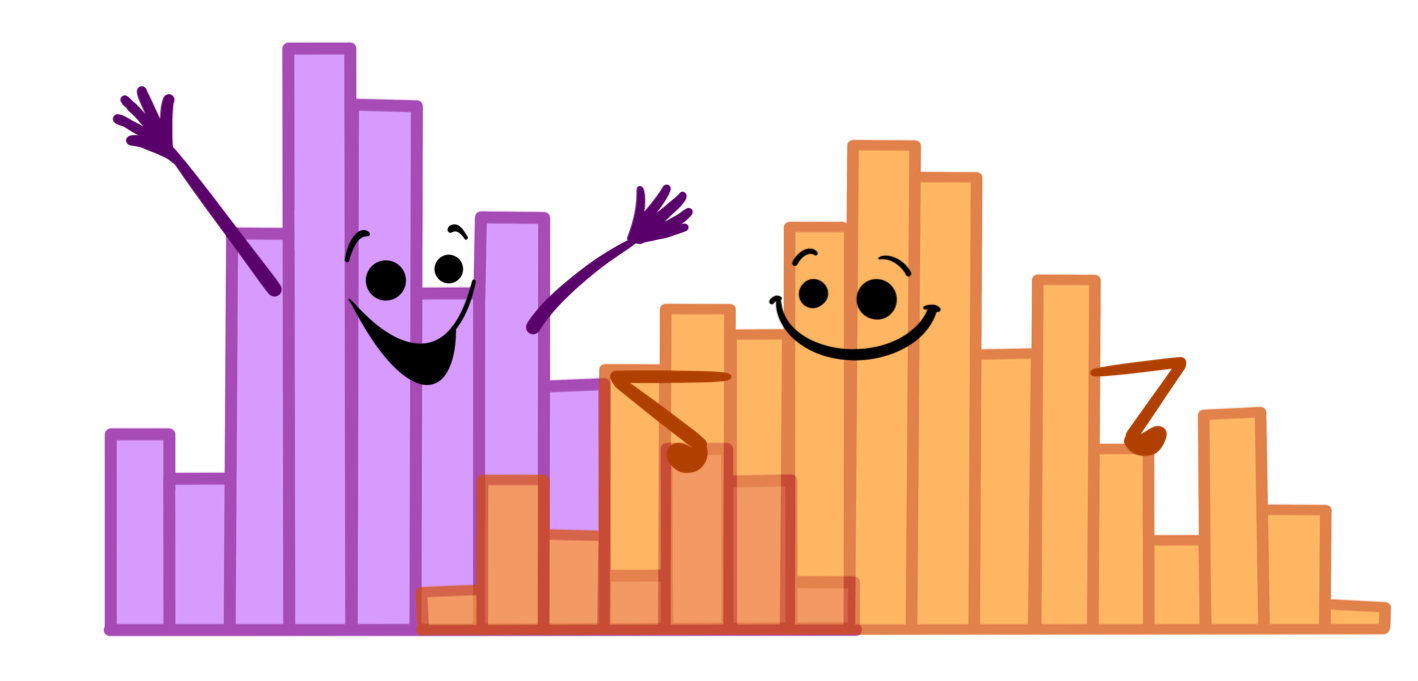
\includegraphics{ex_1.png}
\caption{\label{fig:unnamed-chunk-1}Artwork by \href{https://github.com/allisonhorst}{AllisonHorst}}
\end{figure}

In here you will find links to the written content for each of the separate topics covered as well as the descriptions of the course assessments and projects.

\hypertarget{course-delivery}{%
\section{Course Delivery}\label{course-delivery}}

Data Science is a set of practical research skills grounded in statistics and computer science. Learning a practical skill requires practice! So this course is not a lecture course, it is a `flipped' classroom course with a very strong practical component. In a flipped classroom the onus is on the student to lead their work and practice with the provided materials prior to contact and discussion time with the wider learning group and group mentors. To get the most out of this course you must read the relevant online material before you come to the contact sessions. Contact time will then be an opportunity to discuss the materials and any problems arising with the group and the teacher and to practice and problem solve with others. The aim is that by the end of the course you will have a strong practical grounding in applying data science approaches to research problems that will enhance the biology that you are doing.

\hypertarget{online-materials}{%
\section{Online materials}\label{online-materials}}

The rest of this handbook outlines the online materials provided to you for this course, broken down by the separate topics we will cover. The materials are a mixture of self-led tutorials and interactive challenges or problems to solve.

\hypertarget{course-topics}{%
\section{Course Topics}\label{course-topics}}

We will cover the following topics in data science

\begin{verbatim}
1. Introduction to Genomics
2. Data Exploration and Visualisation
3. Understanding Statistics With Linear Models
4. Introduction to Non-Frequentist Statistics
5. Introduction to Machine Learning
6. Beginning Programming
7. Literate Computation
\end{verbatim}

\hypertarget{course-assessments}{%
\section{Course Assessments}\label{course-assessments}}

The culmination of all this learning and practice will be a written essay and a large group project on which you will be assessed and receive a grade. These will be set at the end of the course and deadlines will be given to you explicitly for each. You will not be formally assessed on other projects, quizzes and challenges occurring through the course.

\hypertarget{intro}{%
\chapter{Why study data science?}\label{intro}}

At first thought, you may imagine that data science is not going to be of much interest to you, your desire and interest is in biology, not computers and mathematics. That may be true but data science is actually going to be one of the main technical themes throughout your entire scientific career and it will help you truly master your science and to become an informed and healthily sceptical interpreter of scientific results. Adding data science as your super power will be of benefit in lots of ways. Learning data science now isn't a tax on your time so that you can get through this M.Sc, it's a valuable investment in your skill set that will help to give you an advantage that will pay definite dividends later. Getting on with data science is like getting on with Jedi training for biologists

\begin{figure}
\centering
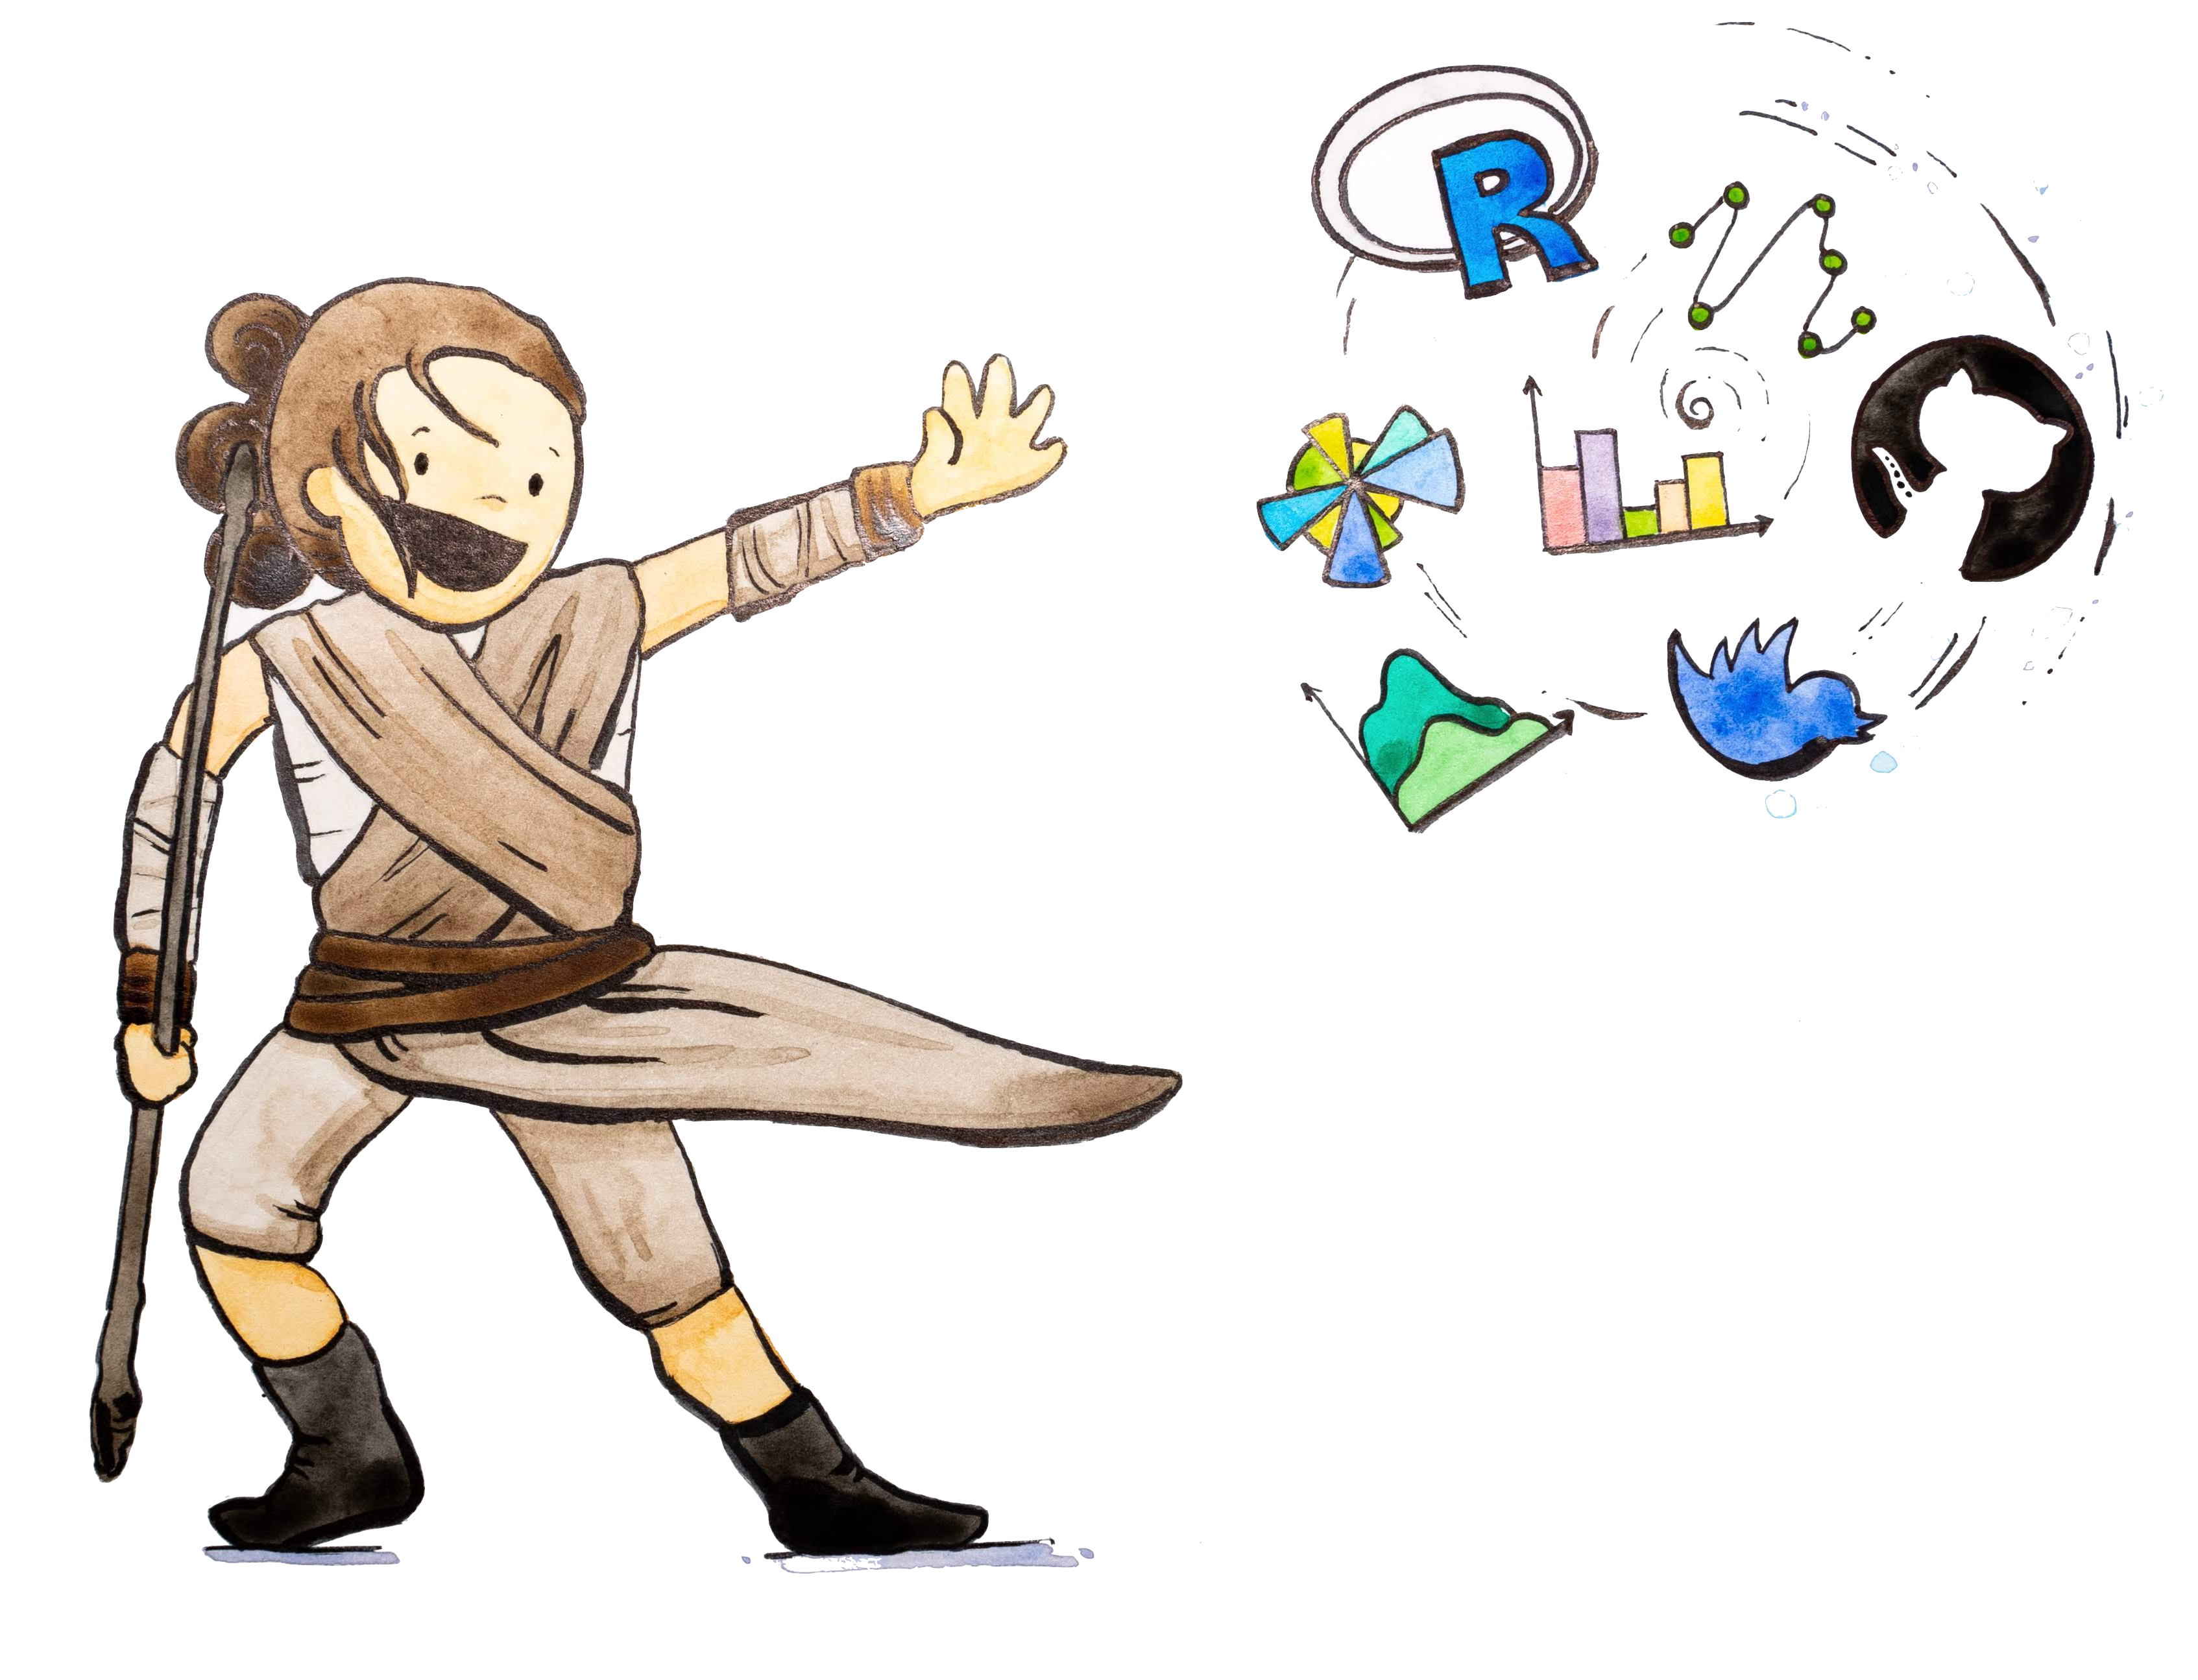
\includegraphics{starwars-rey-rstats.png}
\caption{\label{fig:unnamed-chunk-2}Artwork from \href{https://twitter.com/juliesquid}{@juliesquid} for \href{https://twitter.com/openscapes}{@openscapes} (illustrated by \href{https://twitter.com/allison_horst}{@allison\_horst})}
\end{figure}

\hypertarget{all-experimental-science-is-data-science-sooner-or-later}{%
\section{All experimental science is data science sooner or later}\label{all-experimental-science-is-data-science-sooner-or-later}}

``Data Science'' is a new-ish term that describes an interdisciplinary approach to the practical application of statistics and computer science concepts and tools. The term data scientist is most often applied to people who analyse large amounts of high throughput data full time and have a research or industrial interest in that but the techniques of data science are useful to all researchers, data science is useful to biologists. There is no such thing as a purely lab- or field-based biologist, once our data are collected we must use it in a computer to perform analyses, draw conclusions and draw figures. All modern scientists are at some point a data scientist, irrespective of field and training. Knowledge of data science techniques will therefore underpin everything you do as a scientist at the most fundamental level, from experimental design, data collection, analysis and interpretation of results. A scientist that lacks data science skills will find it very difficult to progress beyond the most basic levels of expertise in experimental analysis.

\hypertarget{biology-is-getting-bigger}{%
\section{Biology is getting bigger}\label{biology-is-getting-bigger}}

All biological disciplines including genomics and genetics, microscopy, biochemistry and proteomics generate volumes of data that are too great to handle by a scientist armed only with a clipboard and spreadsheet, no matter how hard working they are. At the heart of data science are the techniques for dealing with the biggest data sets yet generated and learning just a little about them will stand you in good stead across your entire career.

\hypertarget{data-science-methods-are-21st-century-realisations-of-the-scientific-method}{%
\section{Data science methods are 21st Century realisations of the scientific method}\label{data-science-methods-are-21st-century-realisations-of-the-scientific-method}}

Reproducibility and clear description of process is the keystone of the scientific method, using point and click tools to carry out analyses often do nothing to help you reach this goal but many data science techniques are built with these qualities as a primary design principle and can help to reduce your workload by helping you to do things reproducibly over and again with ease. They can help you share and report on your research and data in a way that is transparent and clear to the reader. They can also help you make the data and analysis you have generated shareable and findable by others.

\hypertarget{introduction-to-genomics}{%
\chapter{Introduction to Genomics}\label{introduction-to-genomics}}

Genomics is a big field with wide use within biology. On the Plant Health M.Sc you are going to learn about a lot of applications of genomics technologies and data science skills underpin \emph{all} of those applications and analysis. So in this first, foundational topic we will look at how to run a basic genomics SNP calling pipeline on the Linux command line. This will include developing the basic skills to use the computer from the command line.

\hypertarget{the-materials}{%
\section{The materials}\label{the-materials}}

As a source for this we will follow the excellent Data Carpentry Genomics Curriculum \url{https://datacarpentry.org/lessons/\#genomics-workshop}. We will do the following two lessons

\begin{enumerate}
\def\labelenumi{\arabic{enumi}.}
\tightlist
\item
  \href{https://datacarpentry.org/lessons/\#genomics-workshop}{Shell Genomics}
\item
  \href{https://datacarpentry.org/wrangling-genomics/}{Data Wrangling and Processing for Genomics}
\end{enumerate}

\hypertarget{for-you-to-do}{%
\section{For you to do}\label{for-you-to-do}}

TODO: Check with SB: about logistics, place and machines and timetables etc
TODO: Schedule this one with contact time first

\hypertarget{data-exploration-and-visualisation}{%
\chapter{Data Exploration and Visualisation}\label{data-exploration-and-visualisation}}

Data exploration and visualisation is the first step in most analyses and the R statistical computing environment is a great tool to work with.

In this topic we will explore techniques in R that allow us answer research questions of our data in a way that follows consistent and straightforward principles. We will learn a data format for keeping our research data organised so that we can readily apply all sorts of useful tools to it. We will also learn a grammar of plots that will allow us to make informative and clear figures. By the end of this you will be comfortable with using R to summarise and work with data frames and create a wide range of plots.

\begin{figure}
\centering

\includegraphics{r_first_then.png}
\caption{\label{fig:unnamed-chunk-3}Artwork by \href{https://github.com/allisonhorst}{@AllisonHorst}}
\end{figure}

\hypertarget{the-materials-1}{%
\section{The materials}\label{the-materials-1}}

For this topic we will use these courses

\begin{enumerate}
\def\labelenumi{\arabic{enumi}.}
\tightlist
\item
  \href{https://danmaclean.github.io/tidyversebook/index.html}{Using dplyr for data analysis}
\item
  \href{https://danmaclean.github.io/ggplotbook/index.html}{Using ggplot2 to producing quality plots}
\end{enumerate}

\hypertarget{for-you-to-do-1}{%
\section{For you to do}\label{for-you-to-do-1}}

TODO: Check with SB: about logistics, place and machines and timetables etc.
TODO: Add in AHorst figures and rewrite challenges, tidy tuesdays?

\hypertarget{understanding-statistics-with-linear-models}{%
\chapter{Understanding Statistics With Linear Models}\label{understanding-statistics-with-linear-models}}

In this topic we will take a look at common statistical methods. Rather than launch into a long list of tests and conditions for use that seems arbitrary we will take advantage of the fact that they are all special cases of a simple tool called a linear model. We will learn about linear models and how to use them to carry out statistical inference. By the end of this topic you will have a clear understanding of how and why to use a linear model in R to carry out most test.

\begin{figure}
\centering
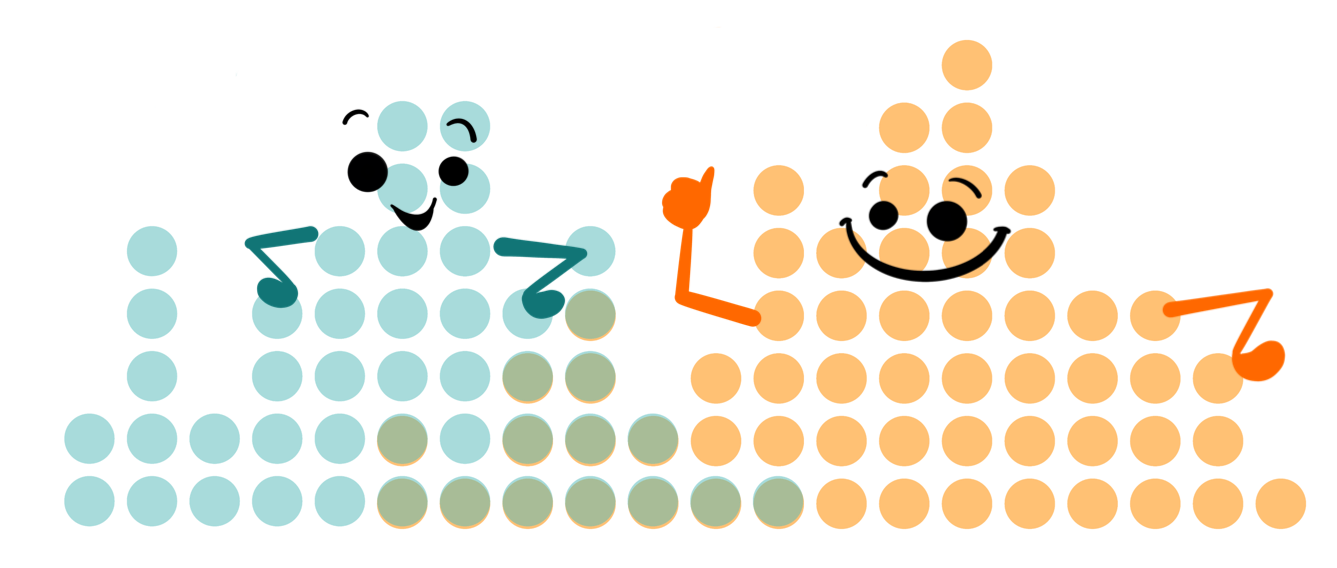
\includegraphics{ex_4.png}
\caption{\label{fig:unnamed-chunk-4}Artwork by \href{https://github.com/allisonhorst}{@AllisonHorst}}
\end{figure}

\hypertarget{the-materials-2}{%
\section{The materials}\label{the-materials-2}}

For this topic we will use this course

\begin{enumerate}
\def\labelenumi{\arabic{enumi}.}
\tightlist
\item
  \href{https://danmaclean.github.io/intro_to_stats/}{Understanding Statistical Thinking With Linear Models}
\end{enumerate}

\hypertarget{for-you-to-do-2}{%
\section{For you to do}\label{for-you-to-do-2}}

TODO: Check with SB: about logistics, place and machines and timetables etc.
TODO: Add in AHorst figures

\hypertarget{introduction-to-non-frequentist-statistics}{%
\chapter{Introduction to Non-Frequentist Statistics}\label{introduction-to-non-frequentist-statistics}}

In this topic we will take a look at alternatives to the standard stattesting tools and models and learn how to make inferences from our data without tests. We will learn to abandon the \(p\)-value as a final arbiter of statistical correctness and see that it is not the only statistic that matters. We will look at using Bayesian inference to make comparisons of hypotheses about our data By the end of this course you will be able to use and interpret standardised effect sizes and create confidence intervals and estimation plots in R. You will be able to use an interpret Bayesian versions of some common statistical tests

\begin{figure}
\centering
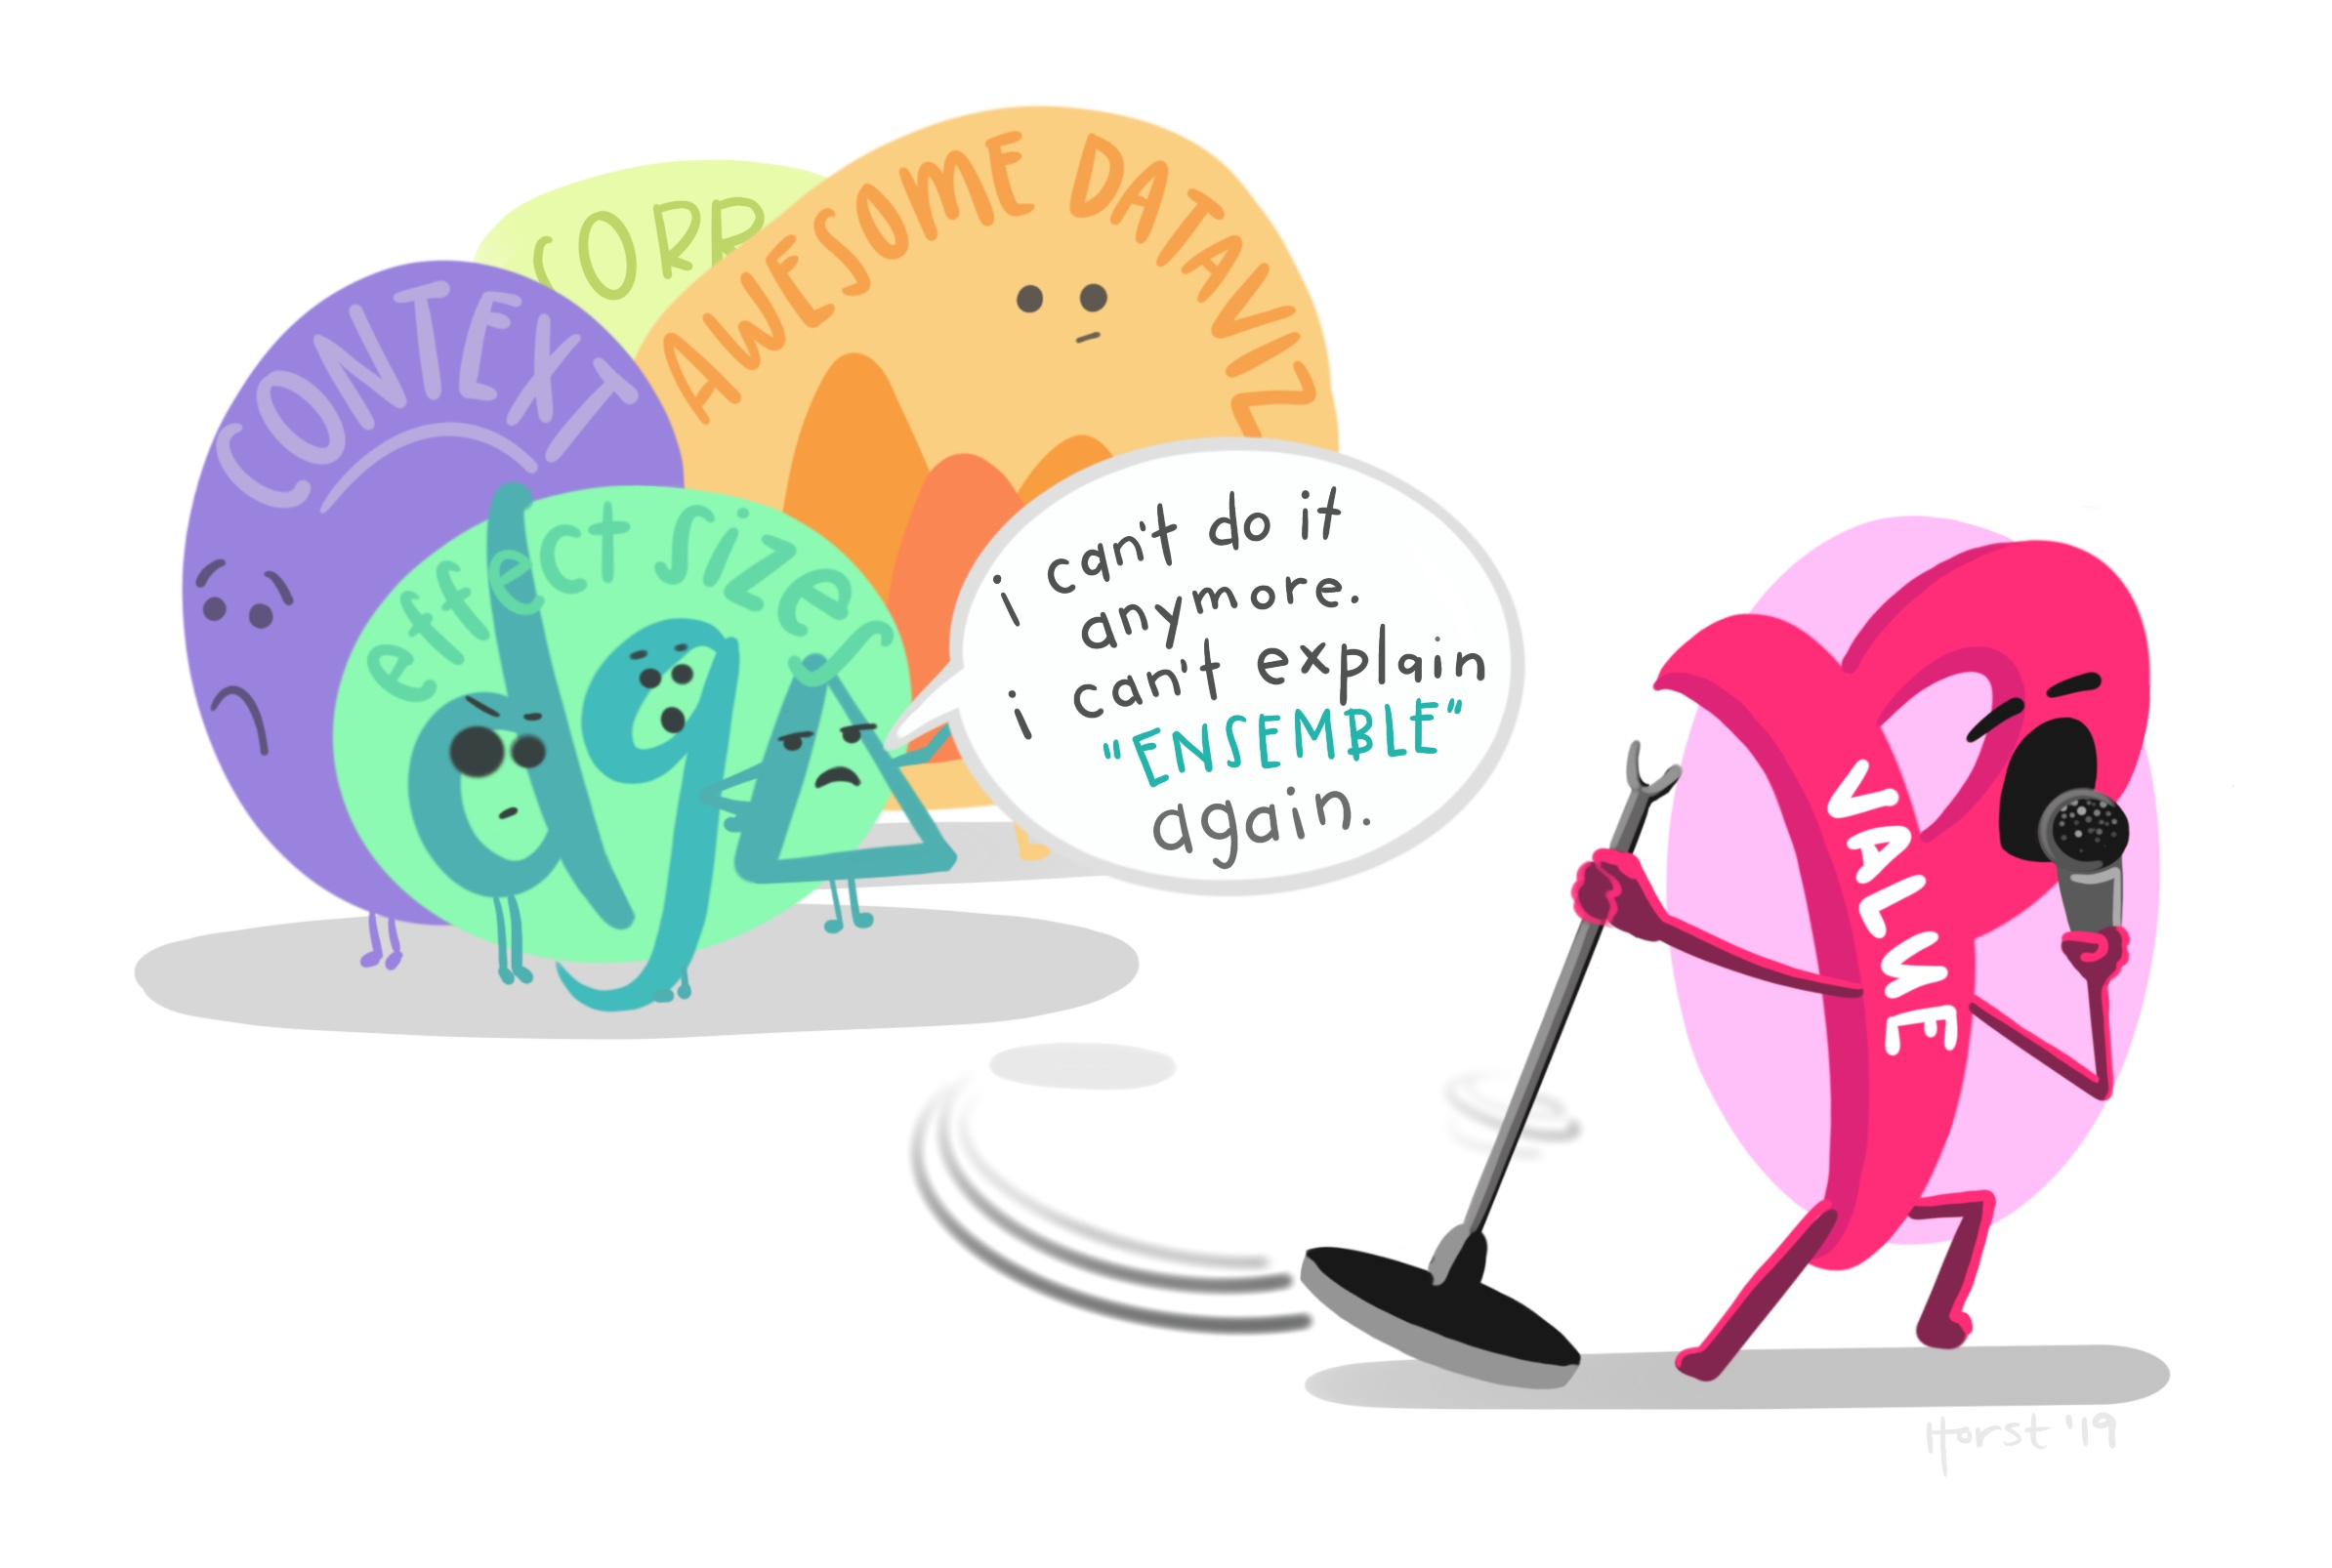
\includegraphics{p_value_mic_hog.jpg}
\caption{\label{fig:unnamed-chunk-5}Artwork by \href{https://github.com/allisonhorst}{@AllisonHorst}}
\end{figure}

\hypertarget{the-materials-3}{%
\section{The materials}\label{the-materials-3}}

For this topic we will use these courses

\begin{enumerate}
\def\labelenumi{\arabic{enumi}.}
\tightlist
\item
  \href{https://danmaclean.github.io/estimation_statistics/}{Estimation Statistics}
\item
  \href{https://danmaclean.github.io/bayes_factors/}{Bayesian Inference with Bayes Factors}
\end{enumerate}

\hypertarget{for-you-to-do-3}{%
\section{For you to do}\label{for-you-to-do-3}}

TODO: Check with SB: about logistics, place and machines and timetables etc.
TODO: Add in AHorst figures and write challenges

\hypertarget{introduction-to-machine-learning}{%
\chapter{Introduction to Machine Learning}\label{introduction-to-machine-learning}}

In this topic we will look at algorithms for performing machine learning as a way of classifying data into groups of similar or dissimilar items. We will use supervised and unsupervised methods in R. We will also study and use some deep learning methods. By the end of this course you will have an understanding of how and when to use classical machine learning in your research and an appreciation of what deep learning methods can achieve and their limitations.

\hypertarget{the-materials-4}{%
\section{The Materials}\label{the-materials-4}}

\href{https://danmaclean.github.io/intro_to_ml/}{Introduction to Machine Learning}

\hypertarget{for-you-to-do-4}{%
\section{For you to do}\label{for-you-to-do-4}}

TODO: Write
TODO: Check with SB: about logistics, place and machines and timetables etc.
TODO: write challenges

\hypertarget{beginning-programming}{%
\chapter{Beginning Programming}\label{beginning-programming}}

Programming is an essential but tricky tool to master for all data scientists. Writing code comes in many guises and in this course up to now we've been writing code for specific tasks with a clear and present idea of what we want to get done. General programming concepts are often harder to grasp because of their generality, so in this topic we will study the general concepts that will allow us to program for a general problem. We will introduce the concepts and learn to use the implementations of them in the Python general purpose programming language. At the end of this topic you will be aware of the most important concepts in programming and how to use them in Python.

\begin{figure}
\centering
\includegraphics{monster_for_loop.png}
\caption{\label{fig:unnamed-chunk-6}Artwork by \href{https://github.com/allisonhorst}{@AllisonHorst}}
\end{figure}

\hypertarget{the-materials-5}{%
\section{The materials}\label{the-materials-5}}

For this topic we will use these courses

\begin{enumerate}
\def\labelenumi{\arabic{enumi}.}
\tightlist
\item
  \href{https://danmaclean.github.io/tao_of_programming/}{A tao of programming}
\item
  \href{https://danmaclean.github.io/programming_with_python/}{Beginning Programming with Python}
\end{enumerate}

\hypertarget{for-you-to-do-5}{%
\section{For you to do}\label{for-you-to-do-5}}

TODO: Check with SB: about logistics, place and machines and timetables etc
TODO: Schedule this one with contact time first

\hypertarget{literate-computation}{%
\chapter{Literate Computation}\label{literate-computation}}

Sitting at a computer and typing commands is only of limited fun. Wrapping commands in scripts is a great way to re-do an analysis without having to type everything in again. But scripts are for computers to read, not humans, so understanding and interpreting an analysis rendered as code alone is not good for general understanding. In this course we'll look at tools and techniques for Literate Computation, a mixing of code, results and human language that results in easily understood executable and re-useable analysis documents. We will also look at tools and strategies for sharing and getting credit for your code and analysis. At the end of this topic you will have a good understanding of how to construct reproducible, reusable and readable analysis documents and how to share them online.

\begin{figure}
\centering
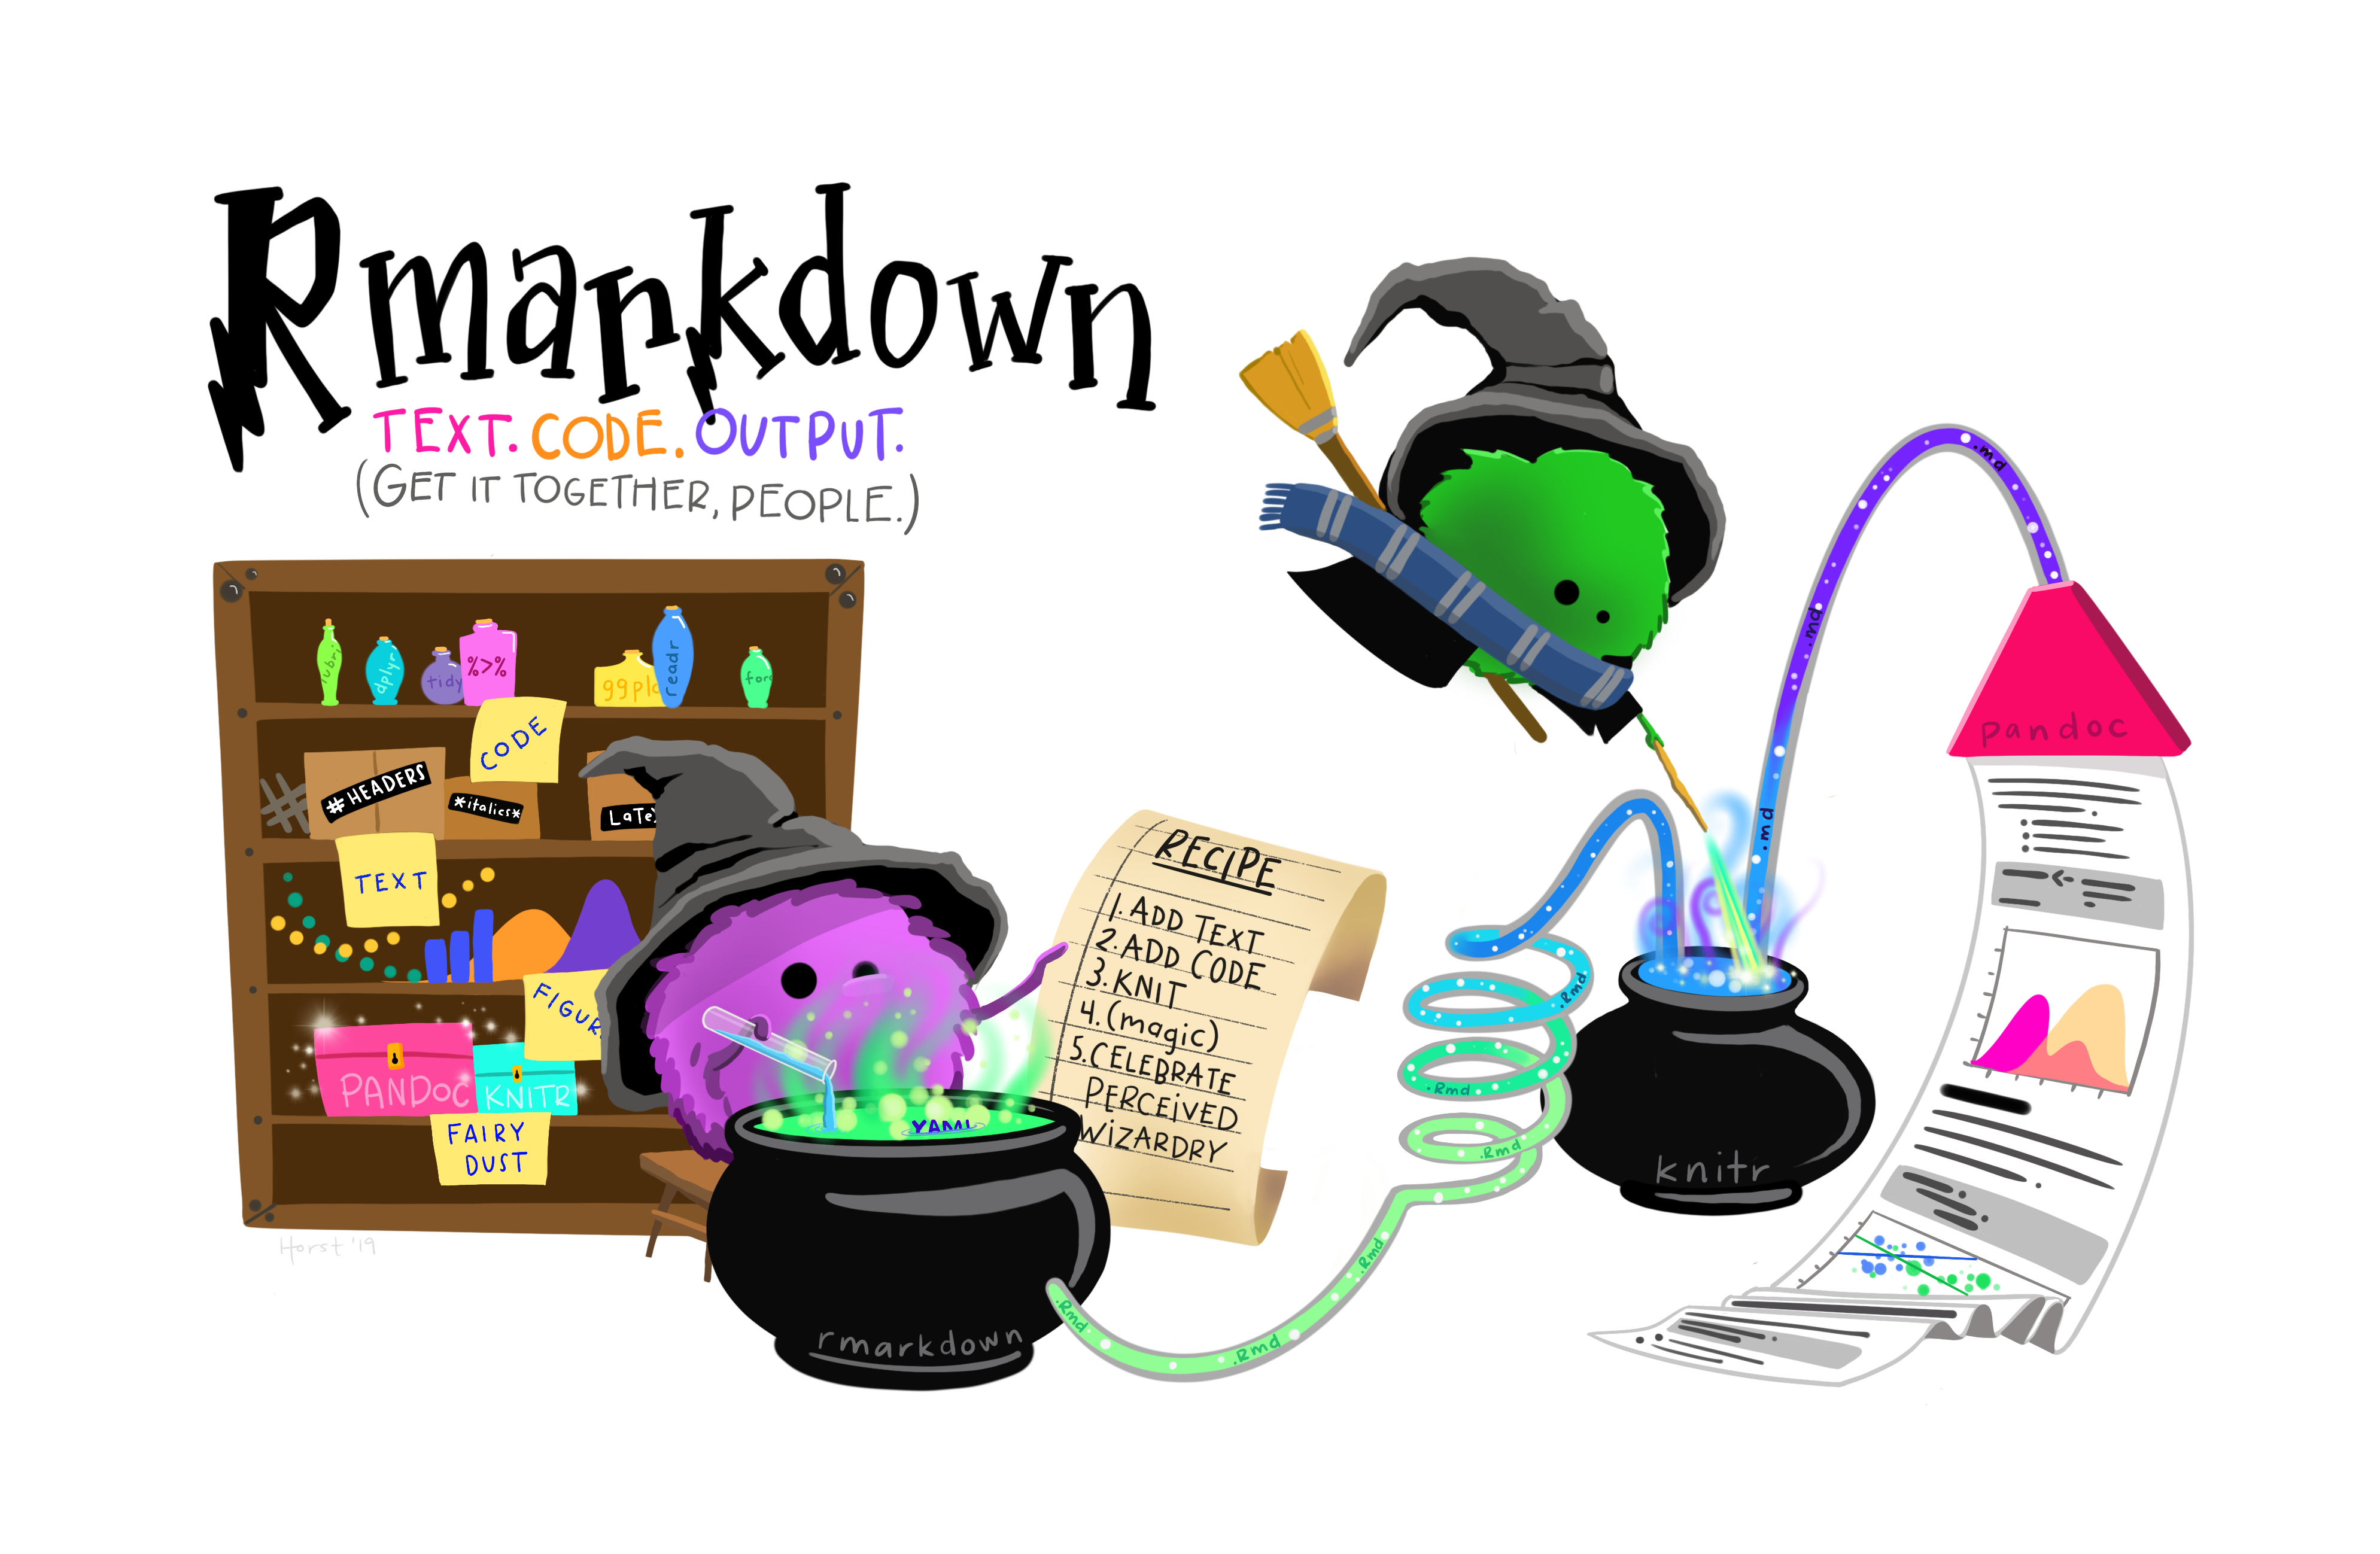
\includegraphics{rmarkdown_wizards.png}
\caption{\label{fig:unnamed-chunk-7}Artwork by \href{https://github.com/allisonhorst}{@AllisonHorst}}
\end{figure}

\hypertarget{the-materials-6}{%
\section{The materials}\label{the-materials-6}}

\hypertarget{for-you-to-do-6}{%
\section{For you to do}\label{for-you-to-do-6}}

TODO: Check with SB: about logistics, place and machines and timetables etc
TODO: Write.

\hypertarget{projects}{%
\chapter{Projects}\label{projects}}

\hypertarget{acknowledgements}{%
\chapter{Acknowledgements}\label{acknowledgements}}

All of the artwork in this repo is by \citep[\textbackslash{}][]{allison_horst}(\url{https://twitter.com/allison_horst}) and is licensed under a Creative Commons Attribution 4.0 International License.

  \bibliography{book.bib,packages.bib}

\end{document}
